\documentclass{article}

% Select the workshop anonymity option required by the final call.
% \usepackage[dblblindworkshop]{neurips_2026}
\usepackage[sglblindworkshop]{neurips_2026}

\usepackage[utf8]{inputenc}
\usepackage[T1]{fontenc}
\usepackage{amsmath}
\usepackage{amssymb}
\usepackage{booktabs}
\usepackage{graphicx}
\usepackage{subcaption}
\usepackage{microtype}
\usepackage{multirow}
\usepackage{tikz}
\usepackage{url}
\usepackage{hyperref}
\usepackage{xcolor}

\graphicspath{{../results/figures/paper/}{../results/figures/}}

\setlength{\textfloatsep}{10pt plus 2pt minus 2pt}
\setlength{\intextsep}{10pt plus 2pt minus 2pt}
\setlength{\abovecaptionskip}{6pt}

% Two hues carry the two levels of every contrast in this paper. Blue marks
% what the binding relation predicts, orange marks what a surface or
% answer-token account predicts. Nothing is coloured for decoration.
\definecolor{bindblue}{HTML}{1F4E79}
\definecolor{surforange}{HTML}{B25000}

\hypersetup{colorlinks=true, linkcolor=bindblue, citecolor=bindblue,
            urlcolor=bindblue}

\title{When Is a Code Representation Semantic?}

\workshoptitle{Interpretability as a Science}

\author{
  Virginia Ceccatelli \\
  University College London \\
  \texttt{v.ceccatelli@ucl.ac.uk}
  \And
  Lorenzo Cavallaro \\
  University College London \\
  \texttt{l.cavallaro@ucl.ac.uk}
}

\begin{document}
\maketitle
\begin{abstract}
Code models perform well on programming tasks, but it is unclear whether this rests on program semantics or on lexical cues that correlate with it, such as identifier spelling, token distance, and indentation. We separate three questions that are often answered with the same evidence, asking whether a program relation is represented beyond surface form, whether that representation survives changes in form, and whether the model's own computation causally uses it. Our construction pairs Python programs differing by one binding-changing character while holding the two probing sites, their token windows, and their separation fixed, so a stated surface reader is uninformative by construction rather than by estimate and scores exactly $0.500$, as does a context-free embedding probe. Against that floor, in DeepSeek-Coder 1.3B and 6.7B, binding is absent at the input, rises within the first few blocks, peaks at $0.981$ and $0.991$ in middle layers, and is partly shed before the output. Frozen probes then locate the failure surface. At 500 inserted tokens inert prose costs little, at $0.914$, while scope-shadowing filler of the same length drives the same probe to $0.576$, so what breaks the representation is added semantic difficulty rather than added distance. Finally, decodability is not use. We fit a rank-1 interchange at the marked use site on one assignment of values to definitions and evaluate it on the crossed assignment, where transporting the same binding demands the opposite token movement. On 280 held-out programs the edit makes DeepSeek-Coder 6.7B emit the value the installed binding selects on $100\%$ of rows in both assignments, while a norm-matched answer direction falls from $27.9\%$ to $4.3\%$ and dose-matched random edits stay near zero. Within this model, layer, and site, the intervention transports which definition is in scope rather than a fixed answer token.
\end{abstract}

\section{Introduction}
\label{sec:intro}

Code models produce convincing programs, but it does not follow that they compute the relations that determine what those programs mean. Equal names usually denote the same variable, definitions and uses tend to be nearby, and indentation usually exposes control structure, so a probe that recovers binding from hidden states may be recovering a relation the model computed, or the text, which those states also contain. The usual response is to estimate how much a shortcut could explain and subtract it. We take a different route, available in code and rarely elsewhere, which is to make the shortcut carry \emph{no information at all} by construction. Every probing example is a pair of Python programs that differ in a single character, at the name an inner assignment writes to. That one character decides whether a later, lexically identical use resolves to the outer definition or the inner one. The two probing sites keep the same token indices, the token windows around them are unchanged, and their separation is unchanged, so the correct answer flips while nothing observable about the text does. Figure~\ref{fig:design} shows the programs that result once this construction is extended for the causal experiment.

This fixes our definition. A program property is \emph{semantic} to the extent that a stated, bounded reader of surface form cannot recover it, and naming that reader is what makes the floor exact. A classifier restricted to the $\pm3$-token windows around both anchors and their bucketed separation must give both members of a pair the same prediction, so on balanced pairs it scores exactly $0.500$ rather than approximately so, and the context-free embedding probe inherits the same floor. Everything above it is information the model's contextual computation introduced. The word \emph{surface} stays relative to this reader, since the construction does not neutralize every computable feature of the source.

We use this leverage for three questions of increasing strength, and our contributions follow that order. \emph{Representation} asks whether a relation is recoverable beyond controlled surface cues, and we give a construction that pins the baseline to exactly $0.500$ by design together with the layerwise profile it licenses (Section~\ref{sec:representation}). \emph{Robustness} asks what that representation is made of, measured with the decoder frozen so that a change in accuracy is a change in the model rather than a refitted probe, and we find it breaks when the underlying problem gets harder rather than when the text gets longer or is spelled differently (Section~\ref{sec:robustness}). \emph{Causal use} asks whether the model's downstream computation reads the relation or merely coexists with it, and we test it with a design that makes transporting a binding and steering an answer predict opposite token movements (Section~\ref{sec:causal}).

\section{Related Work}
\label{sec:related}

Structural probing recovers AST structure, identifiers and namespaces, data flow, and control flow from code models \citep{wan2022capture,hernandez2022astprobe,troshin2022probing,ma2024unveiling}, data flow has been written into pretraining objectives \citep{guo2021graphcodebert}, and models trained on programs acquire latent traces of execution state \citep{jin2024emergent}. These establish \emph{recoverability}, which is where our first question begins rather than ends, because in code the surface form is unusually predictive of the relation. Prior work scores against pooled or unmatched negatives, whereas our baseline is fixed at chance by the construction of the examples, and Section~\ref{sec:representation} shows this changes which relations count as evidence. Control tasks \citep{hewitt2019control} address a related confound and we use them throughout, since they limit what the probe can learn whereas our pairs remove the information from its input. Our intervention is a standard distributed interchange \citep{geiger2023alignments,wu2023boundless,huang2024ravel,zhang2023patching}, and what we add is the identification strategy around it, because a positive interchange at one site cannot separate installing a \emph{relation} from installing an \emph{answer} when both predict the same movement. Binding itself has been studied as attribute attachment to entities \citep{feng2024binding} and as a capability learned by transformers trained from scratch on symbolic programs \citep{wu2025variablebinding}, whereas we resolve which of two competing definitions of the \emph{same} name is in scope, in pretrained models, with arithmetic excluded because it is solved by heuristics that would confound a transport claim \citep{nikankin2024arithmetic}. Finally, semantics-preserving rewriting is a standard robustness probe and long-context work shows models often retain information they do not use \citep{lu2024longcontext}, so we apply rewrites with the decoder frozen and ground truth recomputed per variant. Appendix~\ref{app:related} gives the extended positioning.

\section{Framework and Setup}
\label{sec:setup}

Write $x$ for a program, $s(x)$ for a semantic relation such as which definition a use resolves to, $h_l(x)$ for the model's hidden state at layer $l$, and $y(x)$ for the model's output. The three questions place three different demands on these objects, in increasing order of strength.

\paragraph{Representation.}
A relation is represented at layer $l$ when some probe $g$ drawn from a stated class recovers it from the state,
%
\begin{equation}
  g\big(h_l(x)\big) \;\approx\; s(x),
  \qquad\text{or in information terms}\qquad
  I\big(s(x)\,;\,h_l(x)\big) \;>\; 0 ,
  \label{eq:representation}
\end{equation}
%
scored against a surface-only baseline on the same examples. Naming the class matters, since a rich enough $g$ makes the condition vacuous. Here $g$ ranges over linear classifiers on the pairwise feature of Equation~\ref{eq:feature}. Equation~\ref{eq:representation} is a claim about information present in the state, not about the model using it.

\paragraph{Robustness.}
Let $T$ be a transformation that preserves meaning, so that $s(T(x)) = s(x)$ while the form of the program changes. We fit $g$ once on base programs and evaluate it unchanged on transformed ones, and report the cost of $T$ as
%
\begin{equation}
  \Delta_{\mathrm{rob}}(T)
  \;=\;
  \operatorname{Perf}\!\big(g(h_l(x))\big)
  \;-\;
  \operatorname{Perf}\!\big(g(h_l(T(x)))\big).
  \label{eq:robustness}
\end{equation}
%
Freezing $g$ is what gives Equation~\ref{eq:robustness} its meaning, because a probe refitted on the transformed distribution could recover the relation from whatever cue survives there, and the drop would measure nothing about the model.

\paragraph{Causal use.}
Let $\mathcal{I}(h_l(x), s')$ be an intervention meant to install an alternative semantic state $s'$. Causal use requires the intervened output to match the output of the program that genuinely has $s'$,
%
\begin{equation}
  y\Big(\mathcal{I}\big(h_l(x),\, s'\big)\Big)
  \;\approx\;
  y\big(x \text{ with } s \leftarrow s'\big).
  \label{eq:causal-use}
\end{equation}
%
This is strictly stronger than requiring the output merely to change, that is $y(\mathcal{I}(h_l(x),s')) \neq y(x)$, which an edit that steers toward a fixed token satisfies while transporting nothing. Section~\ref{sec:causal} is built to make those two accounts predict opposite movements.

\paragraph{Probes, controls, and data.}
For anchor positions $i$ and $j$, the probe reads the concatenation
%
\begin{equation}
  \phi(i,j) \;=\; \big[\,h_i \,;\, h_j \,;\, h_i - h_j \,;\, |h_i - h_j|\,\big],
  \label{eq:feature}
\end{equation}
%
which admits position-specific and relational linear evidence without a nonlinear probe. Five-fold cross-validation is grouped by source program, so both members of a counterfactual pair stay in one fold, and we retrain the same classifier on labels shuffled within each program to report \emph{selectivity} \citep{hewitt2019control}. Negatives are reported by difficulty rather than pooled, since easy differently-named negatives would dominate a score they can pass on spelling alone.

We study the frozen, non-instruction-tuned DeepSeek-Coder models at 6.7B, which supplies the main results because it performs the behavioral task the intervention requires, and at 1.3B for cross-scale replication. Synthetic Python generators record exact binding and program-graph structure by construction, and def-use labels are cross-checked against an external static-analysis library. We also evaluate 200 CodeSearchNet Python functions \citep{husain2019codesearchnet}, and every obfuscated variant is executed and kept only if observationally equivalent to its base. Intervention intervals are paired cluster bootstraps over base programs. Appendices~\ref{app:data} and~\ref{app:probes} give alignment, corpus sizes, and the full protocol.

\section{Representation}
\label{sec:representation}

This section answers the weakest of the three questions and the prerequisite for the other two, which is whether the relation is present in the state and where. The alternative it must exclude is that a probe reporting binding is reporting the text, and the context-matched construction excludes that by removing the information rather than bounding it.

Figure~\ref{fig:binding} is the central measurement and its layerwise \emph{shape} is the result rather than any single value. On context-matched pairs the surface reader and the context-free embedding probe both score exactly $0.500$ in both models. The first transformer block reaches $0.557$ in 1.3B and $0.528$ in 6.7B, by layer 3 accuracy is $0.962$ and $0.906$, the peak is $0.981$ at layer 7 in 1.3B and $0.991$ at layer 11 in 6.7B, and the final layer falls back to $0.915$ and $0.934$. Binding is therefore absent from the input representation above the measured floor, is built rapidly under contextual computation, and is partly shed near the output. The models agree on shape and differ only where a scaling account predicts, since 6.7B does less of the work in block 0 and sustains its peak longer over a deeper network. The surface and embedding rows are numerically identical across models, as they must be because neither involves the model, which doubles as a corpus-integrity check. Middle layers therefore carry information about which definition is in scope that no stated surface reader could supply. What does not follow is that the model uses it.

\begin{figure}[t]
\centering
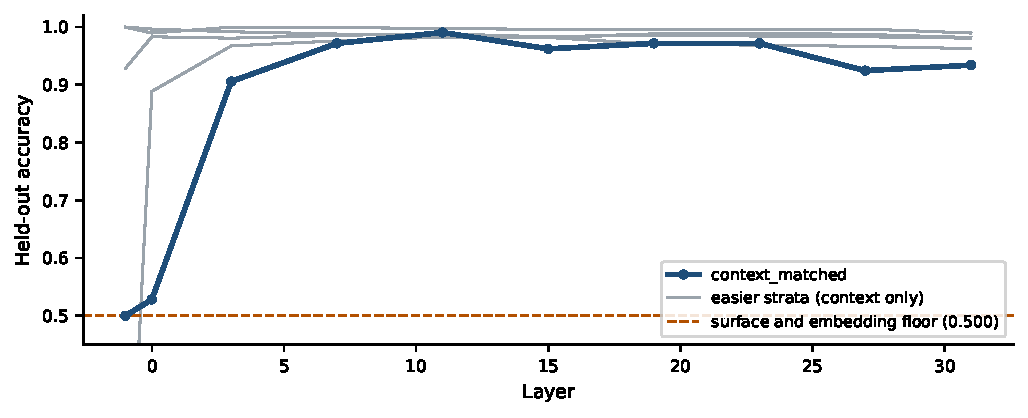
\includegraphics[width=\linewidth]{paper_binding_strata_6.7b.pdf}
\caption{Binding accuracy by layer and negative stratum in DeepSeek-Coder 6.7B. The figure shows a \emph{profile} that no table of best layers conveys. On the decisive \texttt{context\_matched} stratum, accuracy starts at the exact $0.500$ floor the construction pins, rises within the first few blocks, peaks in middle layers, and declines before the output. The easier strata sit near $0.99$ from block 0 onward because their token strings already separate them, so only the matched stratum carries the claim. Figure~\ref{fig:binding-13b} gives the 1.3B panel.}
\label{fig:binding}
\end{figure}

Two further results bound the reading. Def-use edges, whose negatives are matched on token distance, follow the same profile and peak near $0.99$, with the hardest bucket at 50 to 200 tokens holding between $0.96$ and $0.99$. Control dependence is where the criterion bites, since it is decoded almost perfectly yet its surface reader already reaches $0.927$ accuracy and $0.990$ AUC, because the controlling guard is usually the nearest enclosing \texttt{if}, so we report it as a contrast rather than a finding. On 200 CodeSearchNet functions the 6.7B model peaks at AUC $0.978$ for binding and $0.979$ for def-use against surface baselines of $0.673$ and $0.590$, so the layer signature transfers while the exact isolation does not. Appendix~\ref{app:representation} reports both in full.

\section{Robustness}
\label{sec:robustness}

Knowing a relation is decodable does not say what the decoder depends on. Two accounts remain open after Section~\ref{sec:representation}, since the probe may read a stable relational quantity or a feature that merely co-varies with it in the training form. Transformations that preserve the relation and change the form separate the two, measured as $\Delta_{\mathrm{rob}}$ with the probe frozen and ground truth recomputed on each variant.

\paragraph{Distance is cheap, interference is not.}
We insert filler of a measured tokenizer length between a tracked definition and its use, graded by how much it interferes with the relation while leaving it well defined, ranging over inert comment prose, unreachable dead code, fresh decoy names, updates to \emph{other} variables, and nested scopes reusing the \emph{tracked} names. At 500 inserted tokens, 6.7B binding accuracy is $0.914$ under comment prose and $0.576$ under scope shadowing, with the other three conditions between $0.786$ and $0.862$. At 1{,}000 tokens shadowing falls to $0.519$, near chance, while every other filler stays above $0.70$. Because all conditions are matched on inserted token count, only interference varies, so the collapse cannot be attributed to length. Under shadowing the middle layers that normally build binding degrade most while block 0 stays comparatively stable, so the damage lands on the contextual computation rather than on a lexical lookup.

\paragraph{Renaming survives, flattening does not.}
We then apply a cumulative, execution-verified ladder of normalization, consistent renaming of every local, opaque predicates, mixed boolean and arithmetic rewriting, and control-flow flattening. Every transformed program is executed and kept only if observationally equivalent to its base, which licenses treating an accuracy drop as a change in the representation rather than in the label. Best-layer 6.7B binding accuracy moves from $1.000$ after normalization to $0.903$ after renaming, $0.862$ after opaque predicates, $0.857$ after arithmetic rewriting, and $0.770$ after flattening. Read by layer, renaming is the informative case. The embedding and block-0 probes fall well below chance, to $0.379$ and $0.316$, while layers 7 to 15 hold between $0.883$ and $0.903$. Early states encode lexical identity strongly enough that consistent renaming systematically \emph{misleads} the frozen decoder, which is sharper than mere loss of signal, whereas middle states support a relation abstract enough to survive. Flattening damages even the best layer.

\begin{figure}[t]
\centering
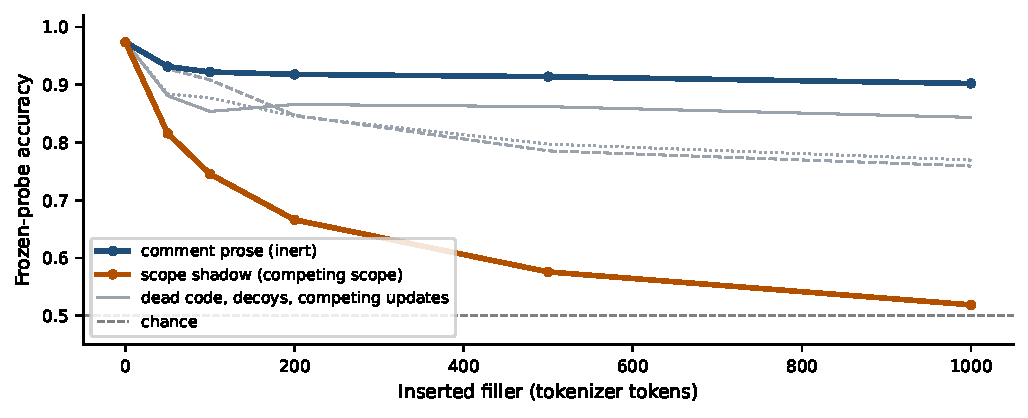
\includegraphics[width=\linewidth]{paper_context_binding_6.7b.pdf}
\caption{Frozen-probe binding accuracy in DeepSeek-Coder 6.7B under inserted context. The \emph{separation} between the conditions is the result. All filler types are matched on inserted token count, so the horizontal axis holds distance constant and the vertical spread is interference alone. Inert prose stays near the unperturbed value while scope shadowing descends to chance, and the intermediate conditions order as their interference predicts.}
\label{fig:robustness}
\end{figure}

Together the two tests place the representation between lexical matching and syntax-independent program analysis. It survives renaming and long inert spans, so the signal is not tied to a spelling or a separation, and it fails under scope shadowing and flattened control flow, so it still depends on how scope and control are written in the source. What does not follow is that the information is destroyed in the failing cases, since a frozen probe can also fail when the representational basis moves.

\section{Causal Use}
\label{sec:causal}

\paragraph{Why decoding does not imply use.}
A probe is an external decoder, so it can recover a quantity the network computed and then ignored, or an incidental byproduct of computing something else. Establishing use means intervening on the internal quantity and checking that behavior follows Equation~\ref{eq:causal-use}. The obvious version of that experiment is ambiguous. Suppose we edit the state at the use site and the answer moves from token $a$ to token $b$, the value the other definition holds. The edit may have installed \emph{which definition is in scope}, and the answer followed, or it may simply encode \emph{emit $b$}, in which case nothing about binding was transported and we have built an answer-steering vector. Ordinary controls cannot separate these, because both accounts predict the same observation.

\paragraph{The four-program design.}
For each base we generate the $2\times2$ design in Figure~\ref{fig:design}. One factor is the \emph{binding}. In the \texttt{source} program the inner assignment writes to a different name, so \texttt{return x} resolves to the outer definition, while in the \texttt{target} program it writes to \texttt{x}, and because Python treats a name assigned anywhere in a function body as local to that body, the same use resolves to the inner definition. The other factor is the \emph{value assignment}, meaning which value sits at each definition. Within a row the two programs differ by exactly one token, at the inner definition's name, and the use token is identical in all four programs at the same index. Crossing the factors is what does the work. In arm \texttt{ab} the outer definition holds $a$ and the inner holds $b$, so switching the binding from outer to inner requires the answer to move from $a$ to $b$. In arm \texttt{ba} the values are exchanged, so the \emph{same} semantic switch requires the answer to move from $b$ to $a$. We fit the intervention only on \texttt{ab} and evaluate it on held-out \texttt{ba}. A direction encoding \emph{emit $b$} must therefore fail on \texttt{ba}, where $b$ is the answer it should be moving away from, whereas a direction carrying which definition is selected must succeed in both.

\begin{figure}[t]
\centering
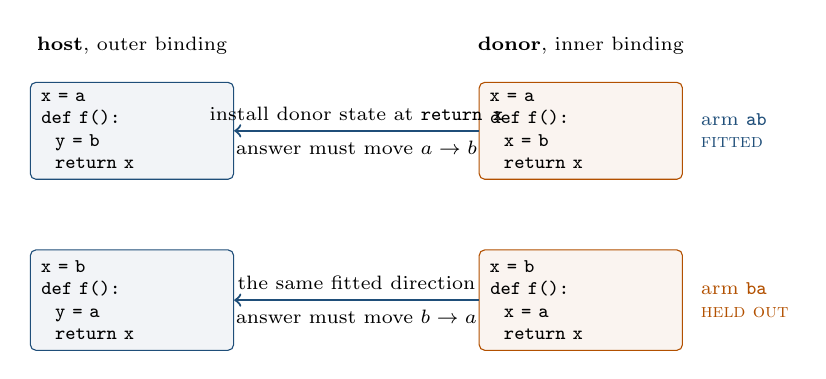
\begin{tikzpicture}[font=\small,
  prog/.style={draw, rounded corners=2pt, inner sep=4pt, font=\ttfamily\scriptsize,
               text width=2.3cm, align=left},
  host/.style={prog, draw=bindblue, fill=bindblue!6},
  donor/.style={prog, draw=surforange, fill=surforange!6},
  lbl/.style={font=\scriptsize},
]
\node[host]  (habs) at (0,0)   {x = a\\def f():\\ \ \ y = b\\ \ \ return x};
\node[donor] (habt) at (5.7,0) {x = a\\def f():\\ \ \ \textbf{x} = b\\ \ \ return x};
\draw[->,thick,bindblue] (habt.west) --
  node[above,lbl,black]{install donor state at \texttt{return x}}
  node[below,lbl,black]{answer must move $a \rightarrow b$} (habs.east);
\node[host]  (hbas) at (0,-2.15)   {x = b\\def f():\\ \ \ y = a\\ \ \ return x};
\node[donor] (hbat) at (5.7,-2.15) {x = b\\def f():\\ \ \ \textbf{x} = a\\ \ \ return x};
\draw[->,thick,bindblue] (hbat.west) --
  node[above,lbl,black]{the same fitted direction}
  node[below,lbl,black]{answer must move $b \rightarrow a$} (hbas.east);
\node[lbl,anchor=south] at (0,0.85)   {\textbf{host}, outer binding};
\node[lbl,anchor=south] at (5.7,0.85) {\textbf{donor}, inner binding};
\node[lbl,anchor=west,align=left,text=bindblue] at (7.1,0)
      {arm \texttt{ab}\\\textsc{fitted}};
\node[lbl,anchor=west,align=left,text=surforange] at (7.1,-2.15)
      {arm \texttt{ba}\\\textsc{held out}};
\end{tikzpicture}
\caption{The crossed causal design, drawn rather than tabulated because the falsification is a relation \emph{between} the two rows. Columns vary which definition \texttt{return x} resolves to, rows vary only which value sits at each definition, and the intervention always installs the donor's inner binding into the host at the use site. The two rows demand opposite token movements for the identical semantic change, so a direction fitted on \texttt{ab} that merely encodes the token $b$ cannot succeed on \texttt{ba}. Bold marks the single differing token.}
\label{fig:design}
\end{figure}

\paragraph{What the rank-1 interchange replaces.}
Let $h_H$ and $h_D$ be the residual-stream states at the marked use token, after layer 8, in the host and donor runs, and let $P=uu^{\top}$ be the orthogonal projection onto a learned unit direction $u$. We replace the host's coordinate along that one direction with the donor's and leave the state otherwise untouched,
\begin{equation}
 h_H^{\mathrm{int}}=(I-P)\,h_H+P\,h_D \;=\; h_H+P\,(h_D-h_H),
 \label{eq:interchange}
\end{equation}
after which the model continues its forward pass normally. Three properties matter. The edit is an interchange rather than a steering vector, so it installs whatever the donor run holds and the realized dose is a measured consequence rather than a tuned choice. It is applied where the two programs are token-identical, at least four tokens downstream of the mutation, so it cannot be transporting an input difference. It is rank 1, so it cannot be smuggling in the whole donor state.

\paragraph{Separating fitting from evaluation.}
Whole base programs, with all four cells, are assigned to either calibration or test, so no test program contributes to any fitted quantity. The direction $u$ is optimized on the \texttt{ab} cells of calibration bases only, ranks $1,2,4,8,16$ are compared on a disjoint calibration split and the smallest successful one is taken, which is rank 1, and the site and layer are likewise chosen on calibration. Everything in Table~\ref{tab:causal-main} is measured on 280 held-out bases, with both arms of a base in the same split so that arm transfer is a within-base contrast rather than generalization to new programs. No \texttt{ba} example enters fitting at any stage.

\paragraph{Prerequisites, and what H4 and H5 add.}
Four conditions are verified first, each closing off a way for the result to be an artifact rather than a finding. Execution and an independently written scope-aware interpreter agree with the generated labels on all 400 bases, with every invariant holding including the arm crossing (H0). The unedited model returns the correctly bound value on $100\%$ of held-out prompts in each cell, so nothing we observe is a capability limit (H1). Binding is decodable at the intervention site at $1.000$ against the measured $0.500$ floor (H2). Replacing the \emph{entire} donor state moves the answer in \emph{both} arms, which sets a ceiling and proves the held-out arm is movable, without which a null on \texttt{ba} could not be distinguished from an arm that is simply not measurable (H3). H4 then asks whether the rank-1 interchange beats its matched controls on the fitted arm, which it does at $189\%$ of that ceiling, though H4 alone is weak evidence since the direction was optimized for that quantity. H5 is the claim, that the same direction transfers unchanged to the held-out assignment where an answer account demands the opposite movement. Table~\ref{tab:causal-main} reports the \emph{installed-answer rate}, whether the full-vocabulary argmax is the value the installed binding selects, which is stricter than a two-way choice because an edit making an unrelated token most likely counts as a failure. Appendix~\ref{app:causal} gives each gate with its threshold.

\begin{table}[t]
\centering
\small
\setlength{\tabcolsep}{5pt}
\caption{Installed-answer rate at the marked use in DeepSeek-Coder 6.7B, layer 8, rank 1, on 280 held-out bases and 560 rows per cell. Each row after the first is an alternative explanation, and the last column names what its result rules out. \emph{Dose} is the realized edit fraction $\|h^{\mathrm{int}}-h\|/\|h\|$, and both random controls are dosed \emph{above} the treatment. Read within a row, where transport is flat across arms and answer steering collapses.}
\label{tab:causal-main}
\begin{tabular}{lrrrl}
\toprule
Intervention & \texttt{ab} & \texttt{ba} & Dose & Rules out \\
\midrule
\textcolor{bindblue}{\textbf{Learned rank-1 interchange}} & \textbf{100.0\%} & \textbf{100.0\%} & .479 & treatment, not a control \\
\midrule
Whole donor state & 85.7\% & 87.9\% & .805 & an unmovable held-out arm \\
Mean donor minus host & 76.1\% & 76.8\% & .711 & need for an optimizer \\
\textcolor{surforange}{Norm-matched answer direction} & 27.9\% & \textcolor{surforange}{4.3\%} & .479 & answer steering \\
Dose-matched random & 2.1\% & 1.8\% & .513 & disruption of this size \\
Rank-matched random & 0.0\% & 0.0\% & .018 & rank-1 edits in general \\
Raw unembedding answer row & 0.0\% & 0.0\% & .479 & a weaker answer account \\
No-op & 0.0\% & 0.0\% & .000 & measurement error \\
\bottomrule
\end{tabular}
\end{table}

\paragraph{What the controls rule out.}
The learned interchange installs the correct value on every held-out row in both arms and never leaves the model on a token that is neither candidate. The decisive comparison is the answer control, which is norm-matched to the treatment and pointed at the token arm \texttt{ab} requires. It works partially where it was aimed, at $27.9\%$, then collapses to $4.3\%$ once the required answer reverses, while the treatment does not attenuate at all, and it knocks the model off both candidates on $9.1\%$ of fitted-arm and $6.4\%$ of held-out rows, which is disruption rather than transport. The remaining rows close the other routes. Random edits dosed \emph{above} the treatment reach only $2.1\%$ and $1.8\%$, so the effect is not perturbation of this size. Whole-state replacement reaches $85.7\%$ and $87.9\%$, so a held-out failure would have been a real negative rather than an untestable cell. The closed-form mean donor minus host direction transports on roughly $76\%$ of rows yet needs dose $.711$ against the learned direction's $.479$, at absolute cosine $0.673$, so the optimizer is isolating a shared axis rather than inventing one.

\paragraph{What follows.}
Within DeepSeek-Coder 6.7B, at layer 8 of the marked use position, under this construction, one direction carries information whose interchange makes downstream behavior follow the installed binding across a reversal of which token that binding implies. That is causal use of the relation rather than merely its presence. It does not follow that binding is globally one-dimensional, that this direction operates at other layers, sites, or templates, or that we have identified the complete mechanism.

\section{Discussion}
\label{sec:discussion}

Read together, the layerwise and robustness results are consistent with a progression from a lexical format, through a relational one, to an output-oriented one. We offer that as an interpretation of the curves rather than a demonstrated decomposition of the network, and the flattening result adds a caution, since whatever the middle layers compute is tied to how scope and control are written in the source rather than to a canonical semantics.

The evidence is narrower than the framing. We study two sizes from one model family, one language, and generated programs emphasizing lexical scope and data flow, and the causal result comes from one model at one layer, one site, and one binding template. The $0.500$ floor is exact for the stated reader and no stronger one, so \emph{surface} is a defined term rather than an absolute, and on natural code the layer signature replicates while the isolation does not. A frozen probe that fails may mean the information is gone or only that its basis moved, which our experiments cannot separate. The rank-1 edit outperforms whole-state replacement, for which we have a plausible but untested account and therefore make no claim. One gate criterion was corrected after the data were seen, and Appendix~\ref{app:h5} gives the verdict under both rules so the reader can discount accordingly.

Interpretability claims become checkable when each stronger word is attached to a stronger falsification. A construction-pinned floor supports \emph{represented}, frozen transformations identify what that representation is made of, and a crossed intervention tests \emph{used}. On that standard, these code models compute scope-sensitive relations whose invariances are limited and measurable, and DeepSeek-Coder 6.7B causally uses binding at the marked use site.

\clearpage
\appendix

\section{Datasets and Construction}
\label{app:data}

\paragraph{Corpora.}
The core representation corpus contains 200 generated binding programs together with additional shadowing templates, from which binding and def-use pairs are extracted, yielding 4{,}015 evaluation rows across 423 program groups. The context study uses 40 base programs crossed with five filler types and insertion targets of 0, 50, 100, 200, 500, and 1{,}000 tokenizer tokens. The cumulative obfuscation ladder uses 40 base programs. The causal study uses 400 base programs with four cells each, for 1{,}600 prompts. All members of a matched family are kept or dropped together, so a caps-based subsample removes whole source-program groups and never individual rows.

\paragraph{Binding pair construction.}
For binding, positive pairs link two identifier occurrences that resolve to the same definition. Negatives are stratified into four kinds of increasing difficulty. \texttt{diff\_name} pairs carry different identifier spellings and are solvable from the text alone. \texttt{distance\_matched} pairs equalize token separation between positives and negatives. \texttt{same\_name\_diff\_binding} pairs share the spelling but resolve to different definitions. \texttt{context\_matched} pairs are the counterfactual construction described in Section~\ref{sec:intro}, in which a second program is token-identical apart from the single character that flips the binding, so that both members carry identical surface features and opposite labels. Reporting the strata separately prevents the easy negatives from dominating the aggregate. Def-use pairs connect a definition to an occurrence reached by that definition, with negatives matched by token distance and reported in buckets of 0 to 10, 10 to 50, and 50 to 200 tokens.

\paragraph{Ground truth and alignment.}
Generators record exact AST-derived semantic events at generation time rather than recovering them afterwards. Def-use extraction is checked against Beniget by equality on straight-line programs and by set inclusion when branching allows several reaching definitions. This audit caught one error in self-referential updates, where a right-hand-side use had been linked to the same-line target rather than to the preceding definition. AST spans are converted to source offsets and then to tokenizer indices, and the recovered token text is compared against the source. The model loader rejects any tokenizer that fails an exact code round trip.

\paragraph{Context variants.}
Filler is inserted between the tracked definition and its use at tokenizer-measured lengths. \texttt{comment\_prose} adds inert English with no executable structure. \texttt{dead\_code} adds unreachable statements. \texttt{lexical\_decoy} introduces fresh identifiers that resemble the tracked names without colliding with them. \texttt{competing\_update} reassigns variables other than the tracked ones. \texttt{scope\_shadow} reuses the tracked names inside a nested scope. All five derive from the same base programs, so the conditions differ only in the content of the insertion, and the frozen probe is scored against ground truth recomputed on each variant.

\paragraph{Obfuscation ladder.}
The ladder is cumulative, so each level includes all previous ones. \texttt{normalize} standardizes formatting. \texttt{rename} consistently replaces every local identifier. \texttt{opaque} inserts branches whose outcome is fixed. \texttt{encode} rewrites arithmetic and boolean expressions. \texttt{flatten} replaces structured control flow with a dispatch loop. Every transformed program is executed and compared against its base, and all variants of a base are retained or rejected together. The guarantee is observational equivalence on the generated executions rather than formal equivalence for all inputs.

\section{Probing Protocol and Controls}
\label{app:probes}

\paragraph{Probe fitting.}
All probes are linear with regularization $C=0.1$, at most 2{,}000 optimization iterations, and at most 20{,}000 examples per task and layer. The pairwise feature $[h_i;h_j;h_i-h_j;|h_i-h_j|]$ permits both position-specific and relational linear evidence without requiring a nonlinear probe, which keeps the probe class stated and fixed as Section~\ref{sec:setup} requires.

\paragraph{Splits.}
Five-fold \texttt{StratifiedGroupKFold} keeps every row from a source program inside a single fold. For the \texttt{context\_matched} stratum this is essential, because the two members of a counterfactual pair belong to the same group and would otherwise leak across folds while carrying opposite labels.

\paragraph{Control task.}
For every pairwise task we retrain the identical classifier on labels shuffled within each source program, which preserves each program's label distribution, and report selectivity as true-label accuracy minus shuffled-label accuracy. On the core corpus, pooled binding selectivity is $0.354$ at layer 11 in 6.7B and def-use selectivity is $0.388$ at layer 3, against control accuracies near chance.

\paragraph{Surface reader.}
The model-free reader receives the token IDs in a $\pm3$ window around both anchors and the bucketed distance between them, and it is trained and evaluated with the same grouped folds as the hidden-state probe. Pooled across strata it reaches $0.798$ accuracy and $0.905$ AUC on binding, which is exactly why the pooled number cannot carry a semantic claim. Per stratum it scores $0.729$ on \texttt{diff\_name}, $0.815$ on \texttt{distance\_matched}, $0.883$ on \texttt{same\_name\_diff\_binding}, and $0.500$ on \texttt{context\_matched}. The last value is fixed by construction, since both members expose identical features and carry opposite labels. This guarantee is specific to the stated reader and does not cover arbitrary whole-program feature engineering.

\paragraph{Uncertainty.}
Accuracy is used for balanced controlled strata. AUC is emphasized on natural code because identifiers there are genuinely predictive and the classes are less balanced. Intervention intervals are paired cluster bootstraps over base programs, and controls are compared on identical rows.

\section{Representation Results}
\label{app:representation}

\begin{figure}[htbp]
\centering
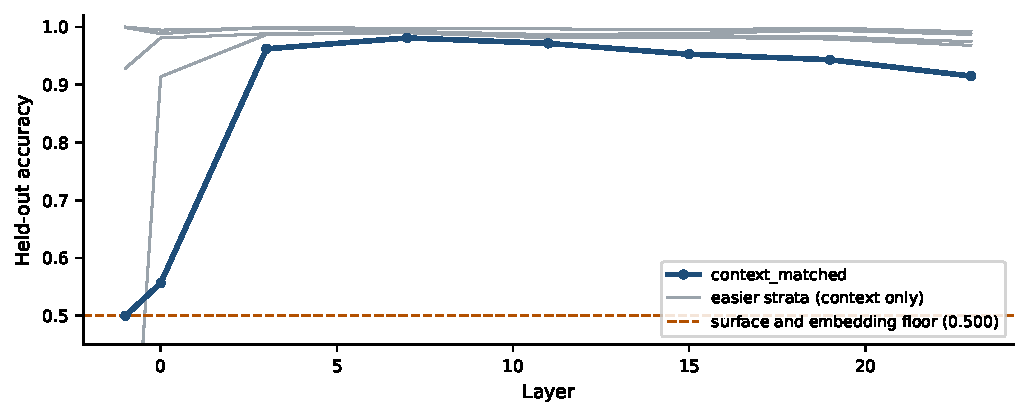
\includegraphics[width=\linewidth]{paper_binding_strata_1.3b.pdf}
\caption{Binding accuracy by layer and negative stratum in DeepSeek-Coder 1.3B, the cross-scale replication of Figure~\ref{fig:binding}. The profile is the same, with the peak reached earlier in absolute layer index and sustained over fewer layers.}
\label{fig:binding-13b}
\end{figure}

\begin{table}[htbp]
\centering
\small
\caption{Context-matched binding accuracy by layer, on 4{,}015 rows across 423 program groups. Layer $-1$ is the context-free embedding. The surface reader and the embedding probe are identical across models because neither involves the model, which is a corpus-integrity check.}
\label{tab:app-binding}
\begin{tabular}{lrrrrrrrrrrr}
\toprule
Model & Surf. & Emb. & L0 & L3 & L7 & L11 & L15 & L19 & L23 & L27 & L31 \\
\midrule
1.3B & .500 & .500 & .557 & .962 & \textbf{.981} & .972 & .953 & .943 & .915 & n/a & n/a \\
6.7B & .500 & .500 & .528 & .906 & .972 & \textbf{.991} & .962 & .972 & .972 & .925 & .934 \\
\bottomrule
\end{tabular}
\end{table}

\begin{table}[htbp]
\centering
\small
\caption{DeepSeek-Coder 6.7B def-use accuracy by token distance between the anchors. Negatives are distance-matched within each bucket, so the hardest bucket is not merely a longer-range version of an easier problem.}
\label{tab:app-defuse}
\begin{tabular}{lrrrrrrrrrrr}
\toprule
Bucket & Emb. & L0 & L3 & L7 & L11 & L15 & L19 & L23 & L27 & L31 \\
\midrule
0 to 10 tokens    & .835 & .982 & .995 & .994 & .996 & .986 & .992 & .990 & .987 & .984 \\
10 to 50 tokens   & .891 & .976 & .989 & .989 & .987 & .986 & .988 & .986 & .985 & .982 \\
50 to 200 tokens  & .923 & .948 & .985 & .974 & .965 & .968 & .979 & .984 & .967 & .962 \\
\bottomrule
\end{tabular}
\end{table}

\begin{table}[htbp]
\centering
\small
\caption{Transfer to 200 AST-parseable CodeSearchNet Python functions, at each model's best layer. The layer signature replicates, but the surface floor is no longer pinned at chance, so these numbers are an upper bound on what transfers semantically.}
\label{tab:app-csn}
\begin{tabular}{llrrrr}
\toprule
Model & Task & Best layer & Accuracy & AUC & Selectivity \\
\midrule
1.3B & Binding  & 3 & .914 & .980 & .329 \\
1.3B & Def-use  & 3 & .912 & .975 & .318 \\
6.7B & Binding  & 7 & .902 & .978 & .308 \\
6.7B & Def-use  & 3 & .911 & .979 & .308 \\
\midrule
\multicolumn{3}{l}{Surface reader, binding} & .685 & .673 & .070 \\
\multicolumn{3}{l}{Surface reader, def-use} & .599 & .590 & $-.025$ \\
\bottomrule
\end{tabular}
\end{table}

\paragraph{Control dependence as a contrast.}
Control dependence asks whether the execution of a statement depends on a particular guard. In 6.7B it is decoded at $0.984$ accuracy and $0.999$ AUC at layer 15, which in isolation looks like strong evidence of semantic computation. Its model-free surface reader, however, reaches $0.927$ accuracy and $0.990$ AUC on the same rows, because the controlling guard is usually the nearest enclosing \texttt{if} and is exposed by neighbouring tokens, nesting depth, and distance. Most of the label is therefore visible without running the model. We include the result because it is a useful falsification of our own criterion. High probe accuracy receives a weaker interpretation whenever a surface-only reader already recovers most of the label, and binding is the stronger case precisely because its controlled reader is pinned at chance.

\section{Robustness Results}
\label{app:robustness}

\begin{table}[htbp]
\centering
\small
\caption{DeepSeek-Coder 6.7B frozen-probe accuracy under inserted context, averaged over evaluated layers. Insertion lengths are measured in tokenizer tokens, so every filler type is matched on length at each column and the differences between rows are interference alone.}
\label{tab:app-context}
\begin{tabular}{llrrrrrr}
\toprule
Task & Filler & 0 & 50 & 100 & 200 & 500 & 1{,}000 \\
\midrule
Binding & \texttt{comment\_prose}    & .974 & .932 & .922 & .918 & .914 & .902 \\
Binding & \texttt{competing\_update} & .975 & .881 & .854 & .866 & .862 & .844 \\
Binding & \texttt{dead\_code}        & .974 & .928 & .908 & .847 & .786 & .759 \\
Binding & \texttt{lexical\_decoy}    & .974 & .884 & .877 & .846 & .797 & .769 \\
Binding & \texttt{scope\_shadow}     & .974 & .816 & .745 & .666 & .576 & .519 \\
\midrule
Def-use & \texttt{comment\_prose}    & .980 & .924 & .908 & .897 & .892 & .881 \\
Def-use & \texttt{competing\_update} & .980 & .895 & .846 & .847 & .868 & .875 \\
Def-use & \texttt{dead\_code}        & .981 & .918 & .876 & .807 & .748 & .712 \\
Def-use & \texttt{lexical\_decoy}    & .981 & .887 & .880 & .843 & .810 & .769 \\
Def-use & \texttt{scope\_shadow}     & .981 & .761 & .722 & .689 & .643 & .596 \\
\bottomrule
\end{tabular}
\end{table}

\begin{table}[htbp]
\centering
\small
\caption{DeepSeek-Coder 6.7B frozen-probe accuracy across the cumulative obfuscation ladder. Best-layer values carry the claim in the main text, and the layer at which the best value occurs is given in parentheses. Layer-averaged values are included because the gap between the two columns is itself informative, showing that the surviving signal is concentrated in a few layers rather than spread across the network.}
\label{tab:app-obf}
\begin{tabular}{lrrrr}
\toprule
Level & Binding, best (layer) & Binding, mean & Def-use, best (layer) & Def-use, mean \\
\midrule
\texttt{normalize} & 1.000 (L7)  & .974 & 1.000 (L7)  & .976 \\
\texttt{rename}    & .903 (L11)  & .726 & .864 (L7)   & .701 \\
\texttt{opaque}    & .862 (L7)   & .722 & .846 (L7)   & .703 \\
\texttt{encode}    & .857 (L7)   & .738 & .833 (L7)   & .717 \\
\texttt{flatten}   & .770 (L31)  & .590 & .890 (L31)  & .598 \\
\bottomrule
\end{tabular}
\end{table}

\begin{table}[htbp]
\centering
\small
\caption{DeepSeek-Coder 6.7B binding accuracy by layer under the obfuscation ladder. The renaming column is the informative one. The embedding and block-0 probes fall far below chance, which means the frozen decoder is systematically misled by consistent renaming rather than merely uninformed, while layers 7 to 15 hold near $0.90$.}
\label{tab:app-obf-layer}
\begin{tabular}{lrrrrr}
\toprule
Layer & \texttt{normalize} & \texttt{rename} & \texttt{opaque} & \texttt{encode} & \texttt{flatten} \\
\midrule
Embedding & .757 & .379 & .459 & .477 & .261 \\
0  & .987 & .316 & .353 & .384 & .175 \\
3  & 1.000 & .624 & .690 & .758 & .440 \\
7  & 1.000 & .883 & .862 & .857 & .615 \\
11 & 1.000 & \textbf{.903} & .848 & .842 & .686 \\
15 & .999 & .886 & .846 & .840 & .729 \\
19 & 1.000 & .875 & .820 & .822 & .748 \\
23 & 1.000 & .837 & .789 & .808 & .724 \\
27 & .999 & .790 & .787 & .799 & .751 \\
31 & .999 & .765 & .770 & .792 & \textbf{.770} \\
\bottomrule
\end{tabular}
\end{table}

\begin{figure}[htbp]
\centering
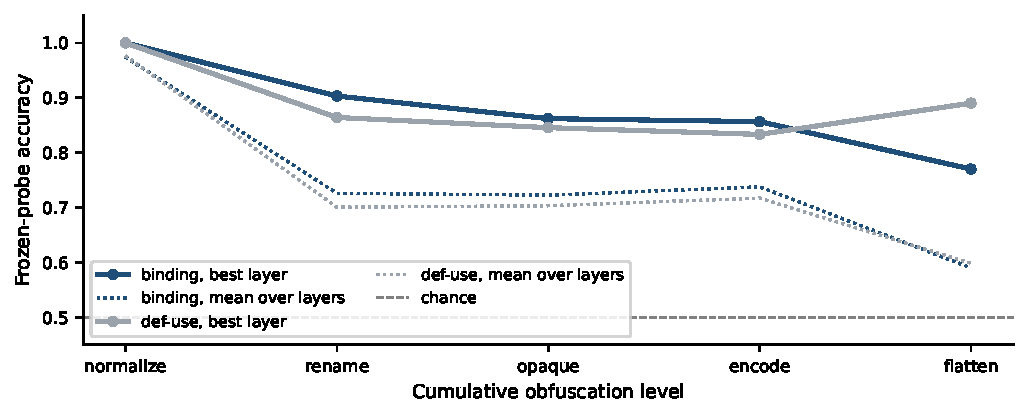
\includegraphics[width=\linewidth]{paper_obfuscation_6.7b.pdf}
\caption{Frozen-probe accuracy across the cumulative obfuscation ladder in DeepSeek-Coder 6.7B, showing best-layer values (solid) and the mean over evaluated layers (dotted). The gap between the two is itself informative, since it shows the surviving signal is concentrated in a few middle layers rather than spread across the network. Cost is roughly flat across \texttt{rename}, \texttt{opaque}, and \texttt{encode}, which change form, and falls again at \texttt{flatten}, which changes structure.}
\label{fig:obf}
\end{figure}

\clearpage
\section{Causal Use in Detail}
\label{app:causal}

\subsection{Programs and invariants}

Each base selects two distinct single-token values $a$ and $b$, an outer name \texttt{x}, and a distinct inner name \texttt{y}. The four program bodies are given below, compressed onto one line each for display, with line breaks and indentation present in the actual prompts.

\begin{center}
\small
\begin{tabular}{ll}
\toprule
\texttt{ab/source} & \texttt{x=a; def f(): y=b; return x} \\
\texttt{ab/target} & \texttt{x=a; def f(): x=b; return x} \\
\texttt{ba/source} & \texttt{x=b; def f(): y=a; return x} \\
\texttt{ba/target} & \texttt{x=b; def f(): x=a; return x} \\
\bottomrule
\end{tabular}
\end{center}

Python treats a name assigned anywhere in a function body as local to that body for the whole body, so the target programs' \texttt{return x} reads the inner assignment while the source programs' identical use reads the outer assignment. Eight invariants are enforced at generation, re-checked independently in verification, and pinned by unit tests. All four prompts share a token length, so every anchor is the same index in all four. Within an arm exactly one token differs, at the inner definition's name. The use token is identical in all four. The use is at least four tokens after the mutation, so no local window on the use can see it. The crossing holds, meaning the answer to \texttt{ab/source} equals the answer to \texttt{ba/target} and the answer to \texttt{ab/target} equals the answer to \texttt{ba/source}. Both values are distinct single tokens. The answer appends exactly one token. No program contains an arithmetic operator, which keeps the required capability a lookup. The crossing is the invariant that makes the held-out arm a falsification rather than a replication, and without it the experiment would prove nothing.

Ground truth is read twice. The generator executes each program, and a separate AST interpreter independently implements Python's function-local scoping rule. All 400 bases agree under both readings and satisfy every invariant, at a measured yield of 400 of 400.

\subsection{Splits and optimization}

Whole base programs, including all four cells, are assigned together to calibration or test, with 120 calibration and 280 test bases. The alignment is optimized only on the \texttt{ab} cells of calibration bases, using 160 training rows. A separate held-out portion of calibration selects the smallest successful rank. For host state $h_H$, donor state $h_D$, and an orthonormal basis $U\in\mathbb{R}^{d\times r}$, the general interchange is
\begin{equation}
 h_H^{\mathrm{int}}=h_H+UU^{\top}(h_D-h_H),
 \label{eq:interchange-general}
\end{equation}
which reduces to Equation~\ref{eq:interchange} at $r=1$. Ranks 1, 2, 4, 8, and 16 were fitted and all five converged, with orthogonality error at most $4.07\times10^{-7}$ and final training losses between $0.0025$ and $0.0086$. Rank 1 was selected as the smallest rank meeting the calibration criterion, and it is the only rank reported. The donor is always the opposite binding within the same value-assignment arm. The intervention is applied at the use anchor after layer 8, and the edited run then proceeds with no further modification.

The site and layer were also chosen on calibration, using the whole-state ceiling as the selection statistic. That scan is informative in its own right. At the use anchor, whole-state replacement produces a logit-difference shift of $+4.781$ at layer 8 and $+3.731$ at layer 12, then falls to $+0.078$ at layer 16 and to zero within noise at layers 20 and 24. At the mutation anchor it reaches only $+0.557$ at layer 8, and at the source definition anchor it is exactly zero, as it must be because host and donor share that state. The causal pathway is therefore concentrated at the use anchor in early-middle layers.

\subsection{Outcome measures}

The primary outcome is the \emph{installed-answer rate}, which asks whether the model's full-vocabulary argmax equals the value the donor binding selects. It is stricter than a two-way choice between the candidates, because an edit that makes an unrelated token most likely counts as a failure. We also report the change in the installed-versus-own logit difference,
\begin{equation}
\Delta_{\mathrm{LD}}=
\big[\log p(y_{\mathrm{inst}})-\log p(y_{\mathrm{own}})\big]_{\mathrm{int}}
-\big[\log p(y_{\mathrm{inst}})-\log p(y_{\mathrm{own}})\big]_{\mathrm{clean}},
\label{eq:delta-ld}
\end{equation}
where $y_{\mathrm{own}}$ is the value the host's use resolves to and $y_{\mathrm{inst}}$ is the value the donor's binding selects. This continuous measure is useful for paired contrasts but is not sufficient evidence of transport. Because clean accuracy is $1.000$, the clean distribution is confident and $\log p(y_{\mathrm{own}})$ sits far above $\log p(y_{\mathrm{inst}})$, so any edit that merely disrupts the state regresses both terms toward the middle and raises $\Delta_{\mathrm{LD}}$ with nothing transported.

\subsection{Prerequisite gates}

\begin{table}[htbp]
\centering
\small
\caption{Prerequisites and decisive tests. Each gate closes off a specific way for the rank-1 result to be uninterpretable rather than negative.}
\label{tab:app-gates}
\begin{tabular}{clp{0.60\linewidth}}
\toprule
Gate & Result & What it establishes \\
\midrule
H0 & Pass & Execution, an independent scope-aware interpreter, and the construction invariants agree on 400 of 400 bases, including the arm crossing. \\
H1 & Pass & Clean behavioral accuracy is $1.000$ overall and $1.000$ in each of the four cells, against thresholds of $0.85$ and $0.75$. \\
H2 & Pass & Binding is decodable at the intervention site at $1.000$ with selectivity $0.524$, against a measured surface floor of $0.500$. \\
H3 & Pass & Whole-state interchange moves both arms, at $+4.781$ on \texttt{ab} and $+4.799$ on \texttt{ba}, with flip rates of $0.857$ and $0.879$. Structural-zero interventions produce exactly zero. \\
H4 & Pass & The rank-1 interchange reaches $189\%$ of the whole-state ceiling on the fitted arm, and all three paired control contrasts clear zero. \\
H5 & Pass & The same direction transfers to the unseen reversed assignment at $100\%$ installed-answer rate, while the answer direction attenuates to an arm ratio of $0.154$. \\
\bottomrule
\end{tabular}
\end{table}

\subsection{Held-out results}

\begin{table}[htbp]
\centering
\small
\caption{Complete held-out causal results at the use anchor, layer 8, rank 1, on 280 base programs and 560 rows per cell. Intervals are paired cluster bootstraps over base programs. \emph{Off-cand.} is the fraction of rows on which the model emits a token that is neither candidate, which separates transport from disruption.}
\label{tab:app-causal}
\begin{tabular}{lrrrrr}
\toprule
Intervention & \texttt{ab} inst. & \texttt{ba} inst. & $\Delta_{\mathrm{LD}}$ (\texttt{ab}) & Off-cand. & Dose \\
\midrule
Learned rank-1 interchange & \textbf{100.0\%} & \textbf{100.0\%} & 9.029 [8.952, 9.108] & 0.0\% & .479 \\
Whole donor state          & 85.7\% & 87.9\% & 4.781 [4.683, 4.878] & 0.0\% & .805 \\
Mean donor minus host      & 76.1\% & 76.8\% & 4.138 [4.025, 4.252] & 0.0\% & .711 \\
Norm-matched answer dir.   & 27.9\% & 4.3\%  & 2.322 [2.157, 2.482] & 9.1\% & .479 \\
Dose-matched random        & 2.1\%  & 1.8\%  & 0.757 [0.691, 0.827] & 0.0\% & .513 \\
Raw unembedding answer row & 0.0\%  & 0.0\%  & 0.039 [0.026, 0.052] & 0.0\% & .479 \\
Rank-matched random        & 0.0\%  & 0.0\%  & $-0.004$ [$-0.005$, $-0.003$] & 0.0\% & .018 \\
No-op                      & 0.0\%  & 0.0\%  & 0.000 [0.000, 0.000] & 0.0\% & .000 \\
\bottomrule
\end{tabular}
\end{table}

\paragraph{Whole state.}
Replacing the entire donor state is the causal ceiling and the proof that both arms are movable. Its installed-answer rate is lower than the rank-1 edit's, which is an observed result and not evidence that whole-state replacement is intrinsically weaker. One possible account is that the donor state contains components that oppose the useful direction, which is consistent with the dose figures but has not been tested.

\paragraph{Answer direction.}
This control is norm-matched to the treatment and points explicitly toward the answer that arm \texttt{ab} requires. It is built from logit-lens rows at the intervention layer rather than from raw unembedding rows, because at layer 8 of 32 the unembedding row is not the direction that moves the output head toward a token. The raw unembedding version is retained in the table for comparison and does nothing in either arm. The lens version works partially where it was aimed and then attenuates $6.5\times$ when the correct answer reverses, which is the behavior an answer-steering account predicts. Unlike the learned interchange, it also produces off-candidate outputs on $9.1\%$ of fitted-arm and $6.4\%$ of held-out rows. One tension is worth stating. Norm-matching this control means a push of $48\%$ of $\|h\|$, and at that magnitude the statement that a direction moves the output toward a token is no longer clearly linear, whereas a unit-norm version would be underpowered. There is no version of this control that is both, which is why the arm-to-arm ratio, a relative statistic with an internal reference, is what we read.

\paragraph{Random controls.}
The dose-matched random direction makes a slightly larger edit than the treatment and almost never produces the installed answer. Rank-matched random and no-op edits stay at zero. Together these rule out rank, numerical noise, and perturbation magnitude as explanations.

\paragraph{Mean difference.}
The normalized average donor minus host difference is a fixed, closed-form direction requiring no optimization. It transports the binding on roughly $76\%$ of rows in both arms, so much of the relevant geometry is shared across examples. It nevertheless moves more of the state and performs worse than the learned direction, and their absolute cosine is $0.673$, so the two are related without being identical. The learned direction captures $59.5\%$ of each state difference against the mean's $88.2\%$, so it is not simply a better-aligned mean.

\paragraph{Implementation checks.}
All 14 checks pass. Structural-zero interventions are exactly $0.00$, which matters because a no-op edit is provably the zero vector and any movement would indicate misaligned hooks, anchors, or dtypes. Patching before the mutation, where host and donor hold the same state, likewise produces exactly zero. The learned basis is orthonormal to $4.07\times10^{-7}$. The whole-state ceiling is alive in both arms. The learned interchange produces no off-candidate outputs. The largest cell contains 280 base programs, which is enough for cluster bootstraps to be informative. Paired training-arm contrasts of the treatment against rank-matched random, dose-matched random, and no-op all have bootstrap intervals above zero, at $+9.033$, $+8.272$, and $+9.029$ respectively.

\subsection{The post-data metric correction}
\label{app:h5}

One gate criterion was changed after the 6.7B data were observed, and we record it here in full because it affects how the causal evidence should be weighed.

H5's third condition requires the explicit \texttt{answer\_direction} control to fail on the held-out arm. If that control does not fail, the design cannot separate an answer encoder from a binding encoder and no verdict is licensed. That condition was originally evaluated on $\Delta_{\mathrm{LD}}$. It is now evaluated on the installed-answer rate, compared against the arm-to-arm ratio that whole-state interchange achieves on the same rows.

The reason we treat this as implementing the pre-registration rather than relaxing it is that the module's design section, written before any 6.7B run, states that $\Delta_{\mathrm{LD}}$ is positively biased and must not be gated on alone, and that every row therefore also records the full-vocabulary argmax, which the gates should read. No gate evaluator read it, so the stated design and the implementation disagreed from the start. The bias is not hypothetical here. Clean accuracy is $1.000$, so any edit that merely disrupts a confident distribution raises $\Delta_{\mathrm{LD}}$ with nothing transported, and the control in question knocked the model off both candidate tokens on $6.4\%$ of held-out rows.

The numbers under both rules are given in Table~\ref{tab:app-h5}. Only the third condition differs. Under the new rule, a control fails on the held-out arm when its \texttt{ba} to \texttt{ab} argmax ratio falls below half the ratio that whole-state interchange achieves on the same rows. The reference is measured on those rows rather than chosen, and the coefficient is the threshold already pre-registered for H5's first condition, so no new free parameter was introduced. What would have made the change illegitimate, and did not happen, is inventing a threshold that the observed $4.3\%$ happens to clear, switching metrics on the first condition as well, where the verdict is unchanged either way, or making the change without leaving the old numbers on the record.

\begin{table}[htbp]
\centering
\small
\caption{H5 under both discriminators, at the use anchor, layer 8, rank 1, on 280 held-out bases. The two rules agree on the first condition and differ only on the third.}
\label{tab:app-h5}
\begin{tabular}{@{}p{0.24\linewidth}p{0.40\linewidth}p{0.29\linewidth}@{}}
\toprule
Condition & Margin rule ($\Delta_{\mathrm{LD}}$) & Argmax rule (installed answer) \\
\midrule
Treatment transfers to \texttt{ba} & $+9.009$ [8.933, 9.089], $188\%$ of ceiling, passes & $100.0\%$, $114\%$ of ceiling, passes \\[2pt]
Answer direction on \texttt{ab}    & $+2.322$ [2.157, 2.482], works & $27.9\%$, works \\[2pt]
Answer direction on \texttt{ba}    & $+0.335$ [0.208, 0.456], interval clears zero, scored as not failing & $4.3\%$, arm ratio $0.154$ against $1.025$, fails \\
\midrule
\textbf{H5 verdict} & \textbf{Fail on the third condition} & \textbf{Pass} \\
\bottomrule
\end{tabular}
\end{table}

\subsection{Scope of the conclusion}

The experiment supports the following claim. At layer 8 of the marked use position in DeepSeek-Coder 6.7B, one learned direction carries information whose interchange makes downstream behavior follow the installed binding across a reversal of value identity, on 280 held-out base programs, against controls that rule out perturbation magnitude, rank, and an explicit answer direction. It does not establish that binding is globally one-dimensional, that the same direction operates at every layer or use site, that the mechanism transfers to natural code or to other languages and model families, or that the learned direction is the model's complete binding mechanism.

\section{Extended Related Work}
\label{app:related}

\paragraph{Probing code models.}
Studies of code-model representations recover token type, AST structure, identifiers, namespaces, data flow, and control flow, generally by fitting a probe on hidden states and reporting accuracy against negatives drawn from the same corpus \citep{wan2022capture,hernandez2022astprobe,troshin2022probing,ma2024unveiling}. The difficulty specific to code is that surface form is unusually predictive of program relations, since two occurrences of the same variable usually share a spelling, a definition and its use are usually close together, and control structure is usually visible in indentation. A probe can therefore score highly by reading the text. Our difference is not a better probe but a better negative. Because each context-matched pair holds a second program that is token-identical apart from the one character that flips the binding, a reader restricted to the stated features must predict identically on both members, so its accuracy is $0.500$ as a property of the construction rather than as an empirical estimate. Section~\ref{sec:representation} shows that this matters in practice, since control dependence is decoded at $0.984$ and is still mostly available to a surface reader at $0.927$.

\paragraph{Probe controls.}
Control tasks \citep{hewitt2019control} ask whether a probe's accuracy reflects the representation or the probe's own capacity, by refitting on randomized labels and reporting the gap. That control constrains the hypothesis class. It does not change what information the input carries, so a probe with low capacity can still read a surface shortcut that is genuinely present. The two controls are therefore complementary rather than substitutable, and we report both, selectivity for the probe and the pinned floor for the input.

\paragraph{Causal abstraction.}
Distributed alignment search and its successors fit a subspace in which interchanging activations between two runs realizes a specified counterfactual, and evaluate with interchange-intervention accuracy and isolation criteria \citep{geiger2023alignments,wu2023boundless,huang2024ravel}. Activation patching has its own methodology for metric choice and site selection \citep{zhang2023patching}. We reuse the operator unchanged. What we contribute is the identification design. In a two-value task, a subspace that installs the correct answer and a subspace that installs a fixed answer token are observationally equivalent at a single value assignment. Crossing the assignment separates them, because the token the binding implies reverses while the binding change does not. This turns an assumption into a measurement, and it is why the answer-direction control is reported as a required discriminator rather than as an optional baseline.

\paragraph{Entity and program binding.}
Feng and Steinhardt study how language models bind entities to attributes in context and identify binding identifiers by causal intervention \citep{feng2024binding}. Wu, Geiger, and Milli\`ere study transformers trained from scratch on symbolic programs with dereference chains and find that program state is not linearly decodable at a single location \citep{wu2025variablebinding}. Our task is different in kind. Attribute retrieval associates distinct entities with distinct properties, whereas lexical scoping requires choosing between two definitions that share a name, so the discriminating information cannot be carried by the identifier. Our setting also differs, since we work in pretrained code models at 1.3B and 6.7B rather than in models trained on the task, and we require no arithmetic at any point, which keeps the behavioral prerequisite a variable lookup that the model performs at $100\%$.

\paragraph{Robustness.}
Semantics-preserving transformation is the standard instrument for asking whether a model tracks meaning rather than form. Our use of it differs in two ways that matter for interpretation. The probe is frozen before any variant is generated, so accuracy changes are attributable to the model rather than to refitting, and the transformations are separated into those that only change form, such as consistent renaming and inert insertion, and those that leave behavior fixed while making the relational problem harder, such as scope shadowing and control-flow flattening. The separation is what produces the finding, since the two classes have clearly different costs. Long-context work provides a useful contrast, in that models can retain information they fail to use \citep{lu2024longcontext}, which is the same representation-versus-use gap that motivates Section~\ref{sec:causal}.

\section{Reproducibility}

The canonical seed is 42. Activation extraction is separated from CPU-only probe fitting, so probes can be refitted without GPU access. Run manifests record arguments and git revisions for every stage, and all paper assets are regenerated from the recorded CSV files. Each causal stage declares its prerequisite gates and refuses to run unless they passed, and any override is recorded permanently in the gate file, in the manifest, and in every affected row. The reported summary and control contrasts are recomputed from the raw per-row records rather than from aggregates written during the GPU run, which is how two aggregation errors in the dose-matched control were caught.

\section{Limitations}

The construction pins the floor for a stated reader, namely $\pm3$ token-ID windows around both anchors plus bucketed distance, and for no stronger one. A cross-position string-equality baseline would be a stricter test and is not yet included.

The representation results cover two model sizes from one family and one language. On natural code the layer signature replicates while the isolation does not, so those numbers bound what transfers semantically rather than measuring it.

Robustness is measured with a frozen decoder, which is what makes a drop attributable to the model. The cost is that a drop cannot distinguish loss of information from a change of representational basis.

Observational equivalence for obfuscated variants is established by executing the generated programs, which is an empirical guarantee on those executions and not a proof for all inputs.

The causal result covers one model, one site, one layer, one rank, and one binding template. The rank-1 edit outperforms whole-state replacement and we do not have a tested explanation. One gate criterion was corrected after the data were seen, as recorded in Appendix~\ref{app:h5}.

\bibliographystyle{plainnat}
\bibliography{references}

\end{document}
